
The most common way of using CMake is via the command-line interface (CLI). CLIs exist in virtually every environment, thus, learning to use CMake in a CLI is essential. In this section, we are going to learn how to perform the most basic CMake operations using the CLI.

Interactions with the CMake CLI can be done by issuing the cmake command in your operating system's terminal, assuming that CMake is installed and the cmake executable is included in your system's PATH variable (or equivalent). You can verify that by issuing cmake in your terminal without any parameters, as shown in the following figure:

\begin{center}
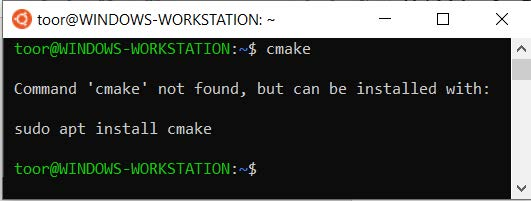
\includegraphics[width=1.\textwidth]{content/1/chapter2/images/1.jpg}\\
Figure 2.1 – Invoking the cmake command
\end{center}

If your terminal is complaining about a missing command, then you should either install CMake (explained in Chapter 1, Kickstarting CMake) or make it discoverable by adding it to your system's PATH variable. Consult your operating system's guide about how to add a path to the system's PATH variable.

After installing CMake and adding it to the PATH variable (if required), you should test whether CMake is usable. The most basic command you can execute in the command line is cmake -{}-version, which allows you to check CMake's version.

\begin{center}
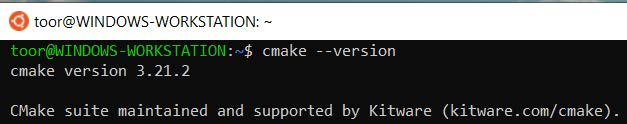
\includegraphics[width=1.\textwidth]{content/1/chapter2/images/2.jpg}\\
Figure 2.2 – Checking CMake's version in the terminal
\end{center}

CMake will output a version string in the form of cmake version <maj.min.rev>. You should see an output that contains the version number of CMake you've installed on your system.

\begin{tcolorbox}[colback=webgreen!5!white,colframe=webgreen!75!black,title=Note]
If the version does not match with the installed one, then you probably have multiple installations of CMake on your system. Since this book contains examples written for CMake version 3.21 and above, it is recommended to have that issue fixed before going any further.
\end{tcolorbox}

After installing CMake, you should install your build system and compiler as well. For Debian-like operating systems (for example, Debian and Ubuntu), this can be easily done by issuing the sudo apt install build-essential command. This package essentially contains gcc, g++, and make.

The CLI usage will be illustrated in the Ubuntu 20.04 environment. Apart from the minor edge cases, the usage is the same in other environments as well. Those edge cases will be mentioned as we go on.

\subsubsubsection{2.2.1\hspace{0.2cm}Learning the basics of the CMake CLI}

The three basic things you should learn about using the CMake CLI are listed here:

\begin{itemize}
\item 
Configuring a CMake project

\item 
Building a CMake project

\item 
Installing a CMake project
\end{itemize}

After learning the basics, you will be able to build and install any CMake project of your choice. Let's get started with configuring.

\hspace*{\fill} \\ %插入空行
\noindent
\textbf{Configuring a project via the CLI}

To configure a CMake project via the command line, you can use the cmake -G "Unix Makefiles" -S <project\_root> -B <output\_directory> construct. The -S argument is used for specifying the CMake project to be configured, whereas -B specifies the configure output directory. Lastly, the -G argument allows us to specify the generator that will be used for the build system generation. The result of the configuration process will be written to <output\_directory>.

As an illustration, let's configure our book's example project in the project root build directory:

\begin{center}
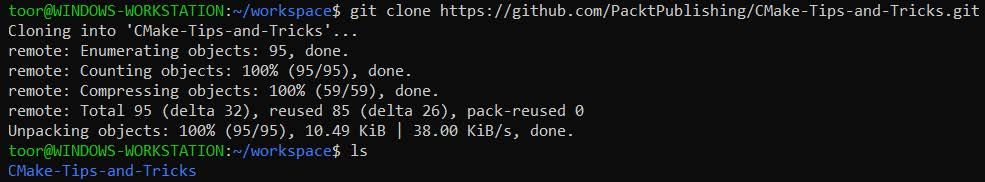
\includegraphics[width=1.\textwidth]{content/1/chapter2/images/3.jpg}\\
Figure 2.3 – Cloning the example code repository
\end{center}

\begin{tcolorbox}[colback=webgreen!5!white,colframe=webgreen!75!black,title=Important Note]
The project must be already present in your environment. If not, clone it via Git by issuing git clone \url{https://github.com/PacktPublishing/CMake-Best-Practices.git} in your terminal.
\end{tcolorbox}

Now go into the CMake-Best-Practices directory and issue cmake -G "Unix Makefiles" -S . -B ./build, as shown in the following figure:

\begin{center}
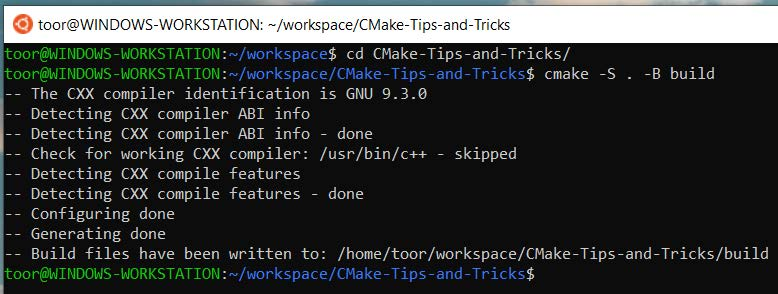
\includegraphics[width=1.\textwidth]{content/1/chapter2/images/4.jpg}\\
Figure 2.4 – Configuring the example code with CMake
\end{center}

This command is like saying to CMake, Use the "Unix Makefiles" (-G "Unix Makefiles") generator to generate a build system for the CMake project in the current directory (-S .) to build (-B ./build) directory.

CMake will configure the project located in the current folder in the build folder. As we omitted the build type, CMake used the Debug build type (the default CMAKE\_BUILD\_TYPE value for the project).

In subsequent sections, we are going to learn about the fundamental settings that are used in the configure step.

\hspace*{\fill} \\ %插入空行
\noindent
\textbf{Changing the build type}

CMake does not assume any build type by default. In order to set the build type, an additional variable named CMAKE\_BUILD\_TYPE must be supplied to the configure command. To supply additional variables, the variable must be prefixed with -D.

To get the Release build instead of Debug, add the CMAKE\_BUILD\_TYPE variable in the configure command, as mentioned previously: cmake -G "Unix Makefiles" -DCMAKE\_BUILD\_TYPE:STRING=Release -S . -B ./build.

\begin{tcolorbox}[colback=webgreen!5!white,colframe=webgreen!75!black,title=Note]
The CMAKE\_BUILD\_TYPE variable only makes sense for singleconfiguration generators, such as Unix Makefiles and Ninja. In multipleconfiguration generators, such as Visual Studio, the build type is a build-time parameter instead of a configuration-time parameter, thus, it cannot be configured by using the CMAKE\_BUILD\_TYPE parameter.
\end{tcolorbox}

\hspace*{\fill} \\ %插入空行
\noindent
\textbf{Changing the generator type}

Depending on the environment, CMake attempts to select an appropriate generator by default. To specify a generator explicitly, the -G argument must be supplied with a valid generator name. For example, if you want to use Ninja as a build system instead of make, you can change it as follows:

\begin{tcblisting}{commandshell={}}
cmake -G "Ninja" -DCMAKE_BUILD_TYPE:STRING=Debug -S . -B ./
build
\end{tcblisting}

The output should be similar to the command output shown in the following figure:

\begin{center}
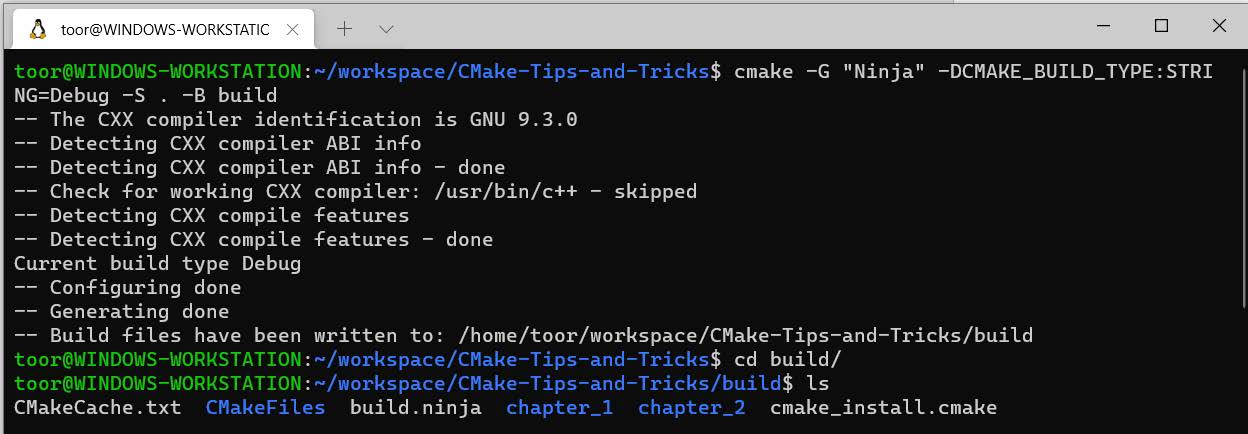
\includegraphics[width=1.\textwidth]{content/1/chapter2/images/5.jpg}\\
Figure 2.5 – Checking the CMake's Ninja generator output
\end{center}

This will cause CMake to generate Ninja build files instead of makefiles.

In order to see all available generator types for your environment, issue the cmake -{}-help command. Available generators will be listed at the end of the Help text generators section, as shown here:

\begin{center}
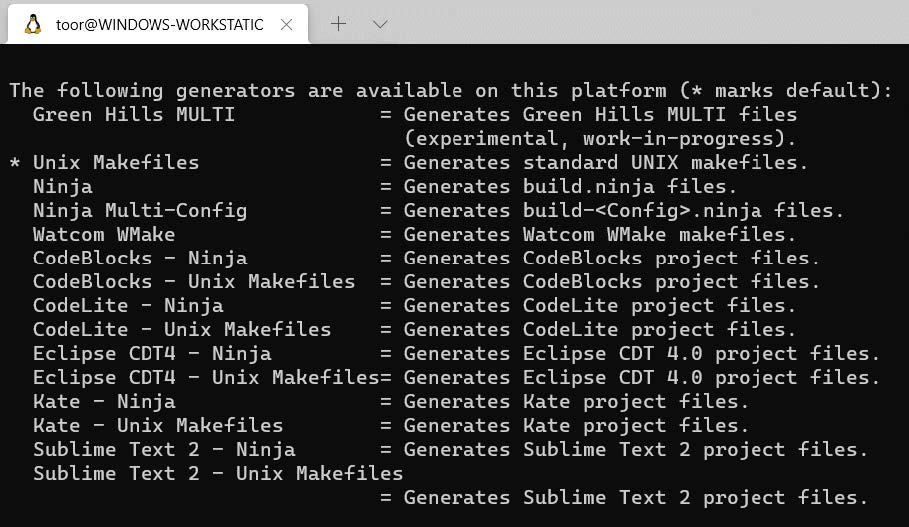
\includegraphics[width=1.\textwidth]{content/1/chapter2/images/6.jpg}\\
Figure 2.6 – List of available generators in help
\end{center}

The generator with one asterisk next to it is the default for the environment you're currently in.

\hspace*{\fill} \\ %插入空行
\noindent
\textbf{Changing the compiler}

In CMake, the compilers to be used are specified on a per-language basis via the CMAKE\_<LANG>\_COMPILER variables. In order to change the compiler for a language, CMAKE\_<LANG>\_COMPILER must be supplied to the Configure command. For a C/C++ project, the variables usually overridden are CMAKE\_C\_COMPILER (C compiler) and CMAKE\_CXX\_COMPILER (C++ compiler). Compiler flags are similarly controlled by the CMAKE\_<LANG>\_FLAGS variable. This variable can be used for holding configuration-independent compiler flags.

As an example, let's try to use g++-10 as a C++ compiler in an environment where it is not the default compiler:

\begin{tcblisting}{commandshell={}}
cmake -G "Unix Makefiles" -DCMAKE_CXX_COMPILER=/usr/bin/g++-10 -S .  
  -B ./build
\end{tcblisting}

Here, we can see g++-10 is used instead of the system's default compiler, g++-9:

\begin{center}
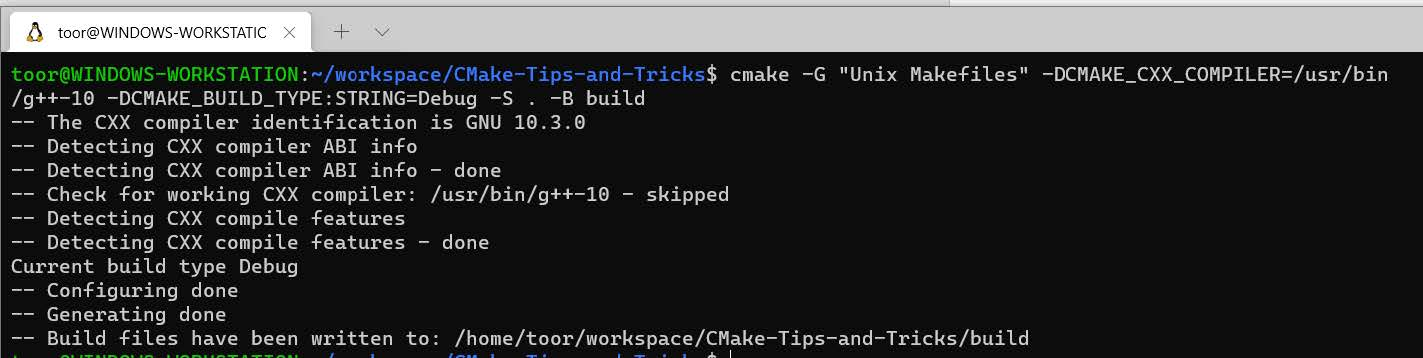
\includegraphics[width=1.\textwidth]{content/1/chapter2/images/7.jpg}\\
Figure 2.7 – Configuring the project using a different compiler (g++-10)
\end{center}

Without the compiler specification, CMake prefers to use g++-9 in this environment:

\begin{center}
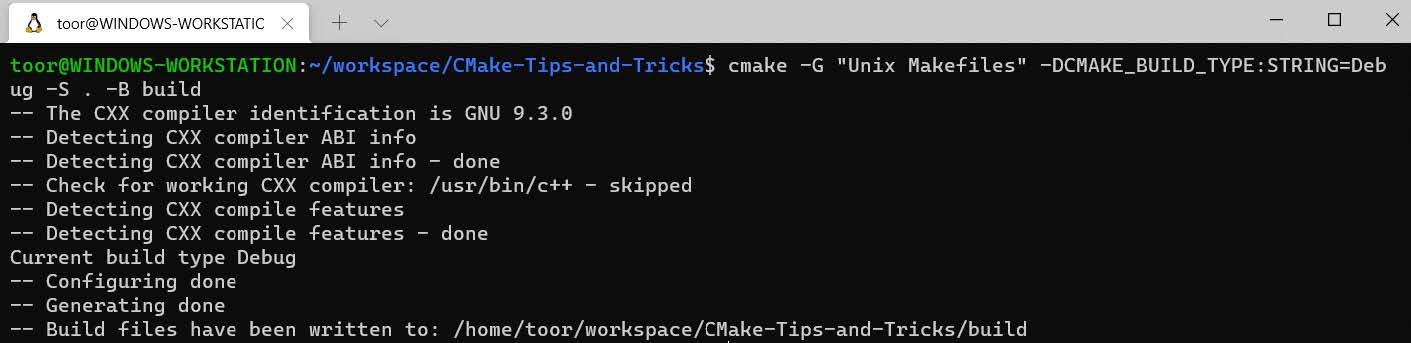
\includegraphics[width=1.\textwidth]{content/1/chapter2/images/8.jpg}\\
Figure 2.8 – Configuring behavior without a compiler preference
\end{center}

\hspace*{\fill} \\ %插入空行
\noindent
\textbf{Passing flags to the compiler}

To illustrate how to specify compiler flags, suppose that you want to enable all warnings and treat them as an error. These behaviors are controlled with -Wall and -Werror compiler flags, respectively, in the gcc toolchain; thus, we need to pass these flags to the C++ compiler. The following code specifies how to do it:

\begin{tcblisting}{commandshell={}}
cmake -G "Unix Makefiles" -DCMAKE_CXX_FLAGS:STRING="-Wall
  -Werror" - S . B ./build S . -B ./build
\end{tcblisting}

We can see the flags specified in the command (-Wall and -Werror) are passed into the compiler in the following example:

\begin{center}
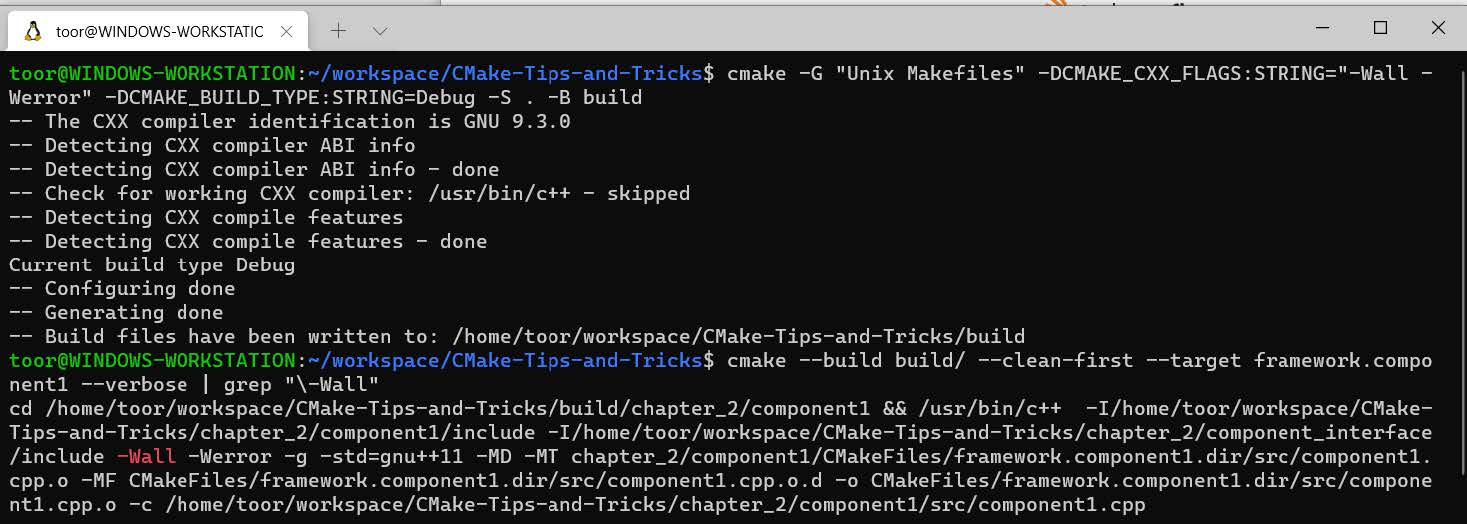
\includegraphics[width=1.\textwidth]{content/1/chapter2/images/9.jpg}\\
Figure 2.9 – Passing flags to the C++ compiler
\end{center}

Build flags can be customized for a per-build type by suffixing them with capitalized build type string. There are four variables for four  different build types, as listed next. They are useful for specifying build types depending on compiler flags. Flags specified in such variables are only valid when the configuration build type matches:

\begin{enumerate}
\item 
CMAKE\_<LANG>\_FLAGS\_DEBUG

\item 
CMAKE\_<LANG>\_FLAGS\_RELEASE

\item 
CMAKE\_<LANG>\_FLAGS\_RELWITHDEBINFO

\item 
CMAKE\_<LANG>\_FLAGS\_MINSIZEREL
\end{enumerate}

In addition to the previous example, if you want to treat warnings as errors only in the Release builds, build type-specific compiler flags allow you to do so.

Here is an example that illustrates the usage of the build type-specific compiler flags:

\begin{tcblisting}{commandshell={}}
cmake -G "Unix Makefiles" -DCMAKE_CXX_FLAGS:STRING="-Wall
  -Werror" -DCMAKE_CXX_FLAGS_RELEASE:STRING="-O3" -DCMAKE_BUILD_
  TYPE:STRING=Debug -S . -B ./build
\end{tcblisting}

Notice that an additional CMAKE\_CXX\_FLAGS\_RELEASE parameter is present in the preceding command. The contents in this variable will only be passed to the compiler when the build type is Release. Since the build type is specified as Debug, we can see the -O3 flag is not present in the flags passed to the compiler, as shown in the following figure:

\begin{center}
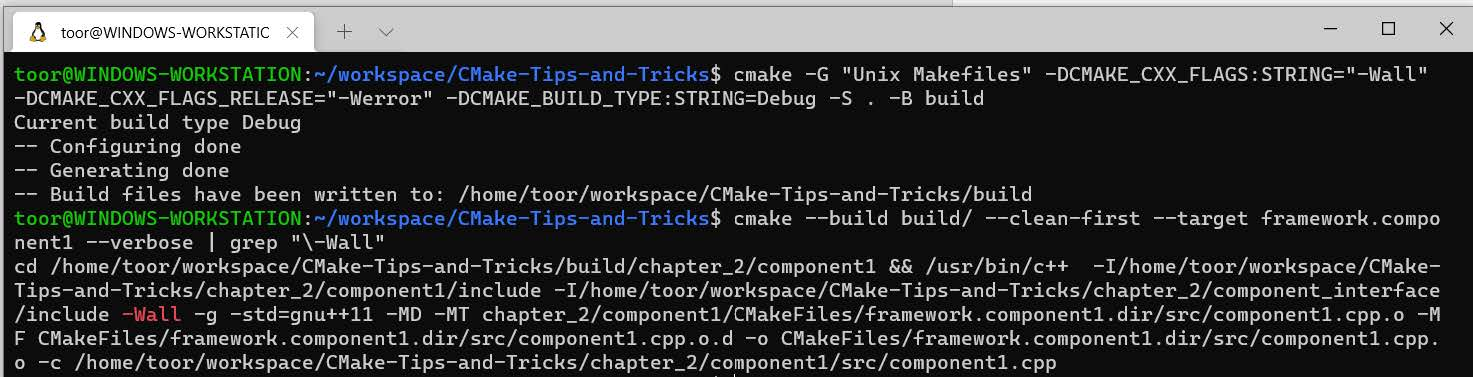
\includegraphics[width=1.\textwidth]{content/1/chapter2/images/10.jpg}\\
Figure 2.10 – Specifying flags based on the build type; the –O3 flag is missing in the Debug build
\end{center}

In Figure 2.10, notice that CMake is issuing a warning about a specified but unused variable, CMAKE\_CXX\_FLAGS\_RELEASE. This confirms that the CMAKE\_CXX\_FLAGS\_RELEASE variable is not used in the Debug build type. When the build type is specified as Release, we can see that the -O3 flag is present:

\begin{tcblisting}{commandshell={}}
cmake -G "Unix Makefiles" -DCMAKE_CXX_FLAGS:STRING="-Wall
-Werror" -DCMAKE_CXX_FLAGS_RELEASE:STRING="-O3"
-DCMAKE_BUILD_TYPE:STRING= "Release" -S . -B ./build
\end{tcblisting}

In this line, you are saying to CMake, Configure the CMake project located at the current directory to build/folder using the "Unix Makefiles" generator. For all build types, pass the -Wall flag to the compiler unconditionally. If the build type is Release, pass the -O3 flag as well.

Here is the output of the command when the build type is set to Release:

\begin{center}
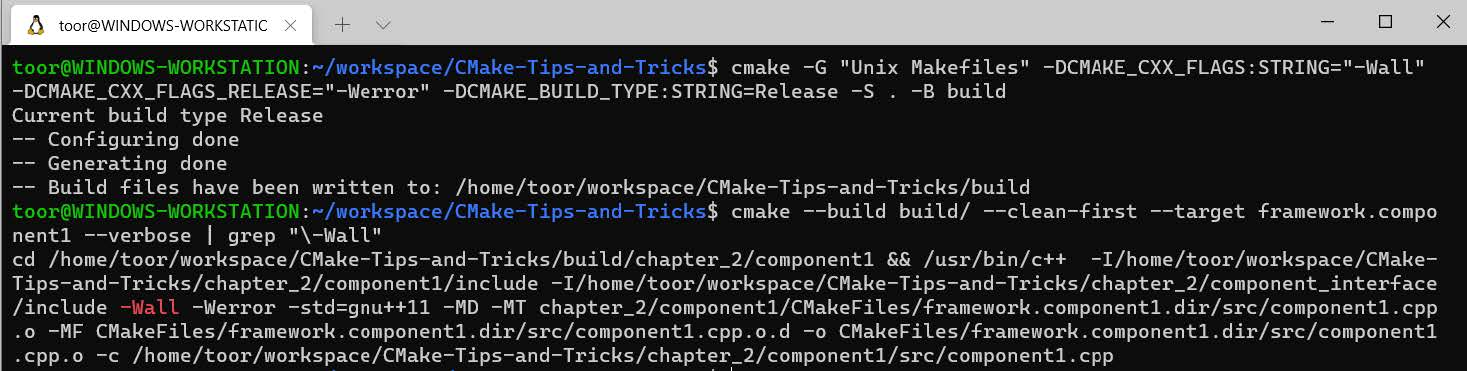
\includegraphics[width=1.\textwidth]{content/1/chapter2/images/11.jpg}\\
Figure 2.11 – Specifying flags based on build type; the -O3 flag is present in the Release build
\end{center}

In Figure 2.11, we can confirm that the -O3 flag is passed to the compiler as well. Be aware that even though RelWithDebInfo and MinSizeRel are also release builds, they are separate from the Release build type, and so flags specified in the CMAKE\_<LANG>\_FLAGS\_RELEASE variable will not apply to them.

\hspace*{\fill} \\ %插入空行
\noindent
\textbf{Listing cached variables}

You can list all the cached variables by issuing the cmake -L ./build/ command (see Figure 2.12). This, by default, does not show the advanced variables and help strings associated with each variable. To show them as well, use the cmake -LAH ./build/ command instead.

\begin{center}
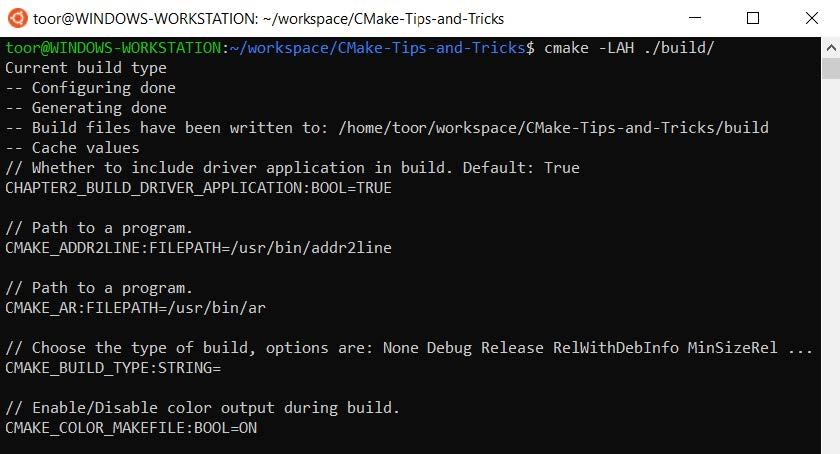
\includegraphics[width=1.\textwidth]{content/1/chapter2/images/12.jpg}\\
Figure 2.12 – List of cached variables dumped by CMake
\end{center}

\hspace*{\fill} \\ %插入空行
\noindent
\textbf{Building a configured project via CLI}

To build the configured project, issue the cmake -{}-build ./build command. This command tells DCMake to Build the CMake project already configured in the build folder.

You can also equivalently issue cd build \&\& make. The benefit of using cmake -{}-build is that it saves you from invoking build system-specific commands. It is especially helpful when building CI pipelines or build scripts. In this way, you can change your build system generator without changing your build command.

You can see an example output for the cmake --build ./build command in the following example:

\begin{center}
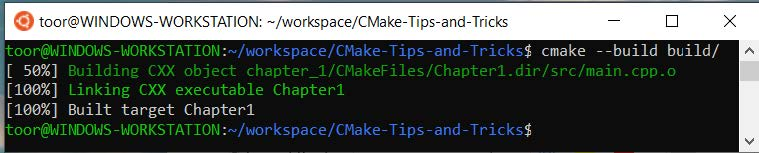
\includegraphics[width=1.\textwidth]{content/1/chapter2/images/13.jpg}\\
Figure 2.13 – Building a configured project
\end{center}

\hspace*{\fill} \\ %插入空行
\noindent
\textbf{Building in parallel}

You can also customize build time details while issuing the build command. The most prominent build time configuration is the number of jobs that will be used to build the project. To specify job count, append -{}-parallel <job\_count> to your cmake -{}-build command.

To build in parallel, issue cmake -{}-build ./build -{}-parallel 2, where the number 2 specifies the job count. The recommended number of jobs for a build system is, at most, one job per hardware thread. In multi-core systems, it is also recommended to use at least one less than the available hardware thread count to not affect the system's responsivity during the build process.

\begin{tcolorbox}[colback=webgreen!5!white,colframe=webgreen!75!black,title=Note]
You can usually use more than one job per hardware thread and get faster build times since the build process is mostly I/O bound, but your mileage may vary. Experiment and observe.

Also, some of the build systems, such as Ninja, will try to utilize as many hardware threads as are available in the system, so it is redundant to specify the job count for such build systems if your target is to use all hardware threads in your system. You can retrieve the hardware thread count by issuing the nproc command in Linux environments.
\end{tcolorbox}

It is a good practice not to use fixed values for environment-dependent variables in the commands that are expected to be invoked in different environments, such as CI/CD scripts and build scripts. Here is an example build command that utilizes nproc to determine the number of parallel jobs dynamically:

\begin{tcblisting}{commandshell={}}
cmake --build ./build/ --parallel $(($(nproc)-1))
\end{tcblisting}

Let's observe how different job counts affect the build time. We will use the time tool to measure how long each command invocation is. The environment details are as follows:

\begin{itemize}
\item 
OS: Ubuntu 20.04.3 LTS (Focal Fossa)

\item 
CPU: AMD Ryzen Threadripper 1950X 16-Core Processor (32 hardware threads)

\item 
RAM: 32 GB
\end{itemize}

With one job (--parallel 1), the build time result would be as follows:

\begin{center}
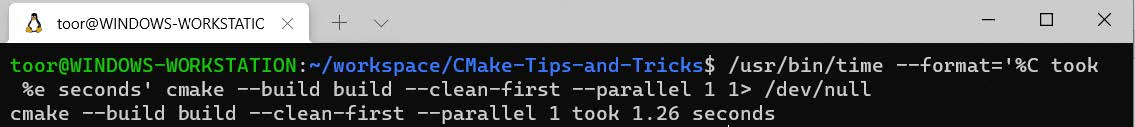
\includegraphics[width=1.\textwidth]{content/1/chapter2/images/14.jpg}\\
Figure 2.14 – Parallelized build time result with one job
\end{center}

The build time result with two jobs (-{}-parallel 2) would be as follows:

\begin{center}
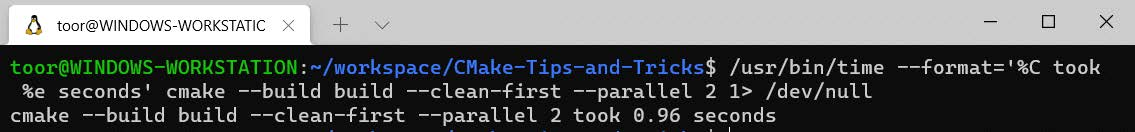
\includegraphics[width=1.\textwidth]{content/1/chapter2/images/15.jpg}\\
Figure 2.15 – Parallelized build time result with two jobs
\end{center}

This is the build time result with four jobs (-{}-parallel 3):

\begin{center}
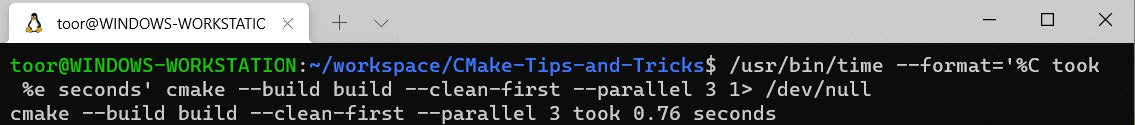
\includegraphics[width=1.\textwidth]{content/1/chapter2/images/16.jpg}\\
Figure 2.16 – Parallelized build time result with three jobs
\end{center}

This is the build time result with four jobs (-{}-parallel 4):

\begin{center}
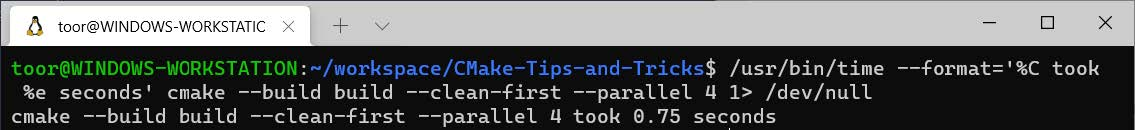
\includegraphics[width=1.\textwidth]{content/1/chapter2/images/17.jpg}\\
Figure 2.17 – Parallelized build time result with four jobs
\end{center}

Even though invoked on a very simple project, we can clearly see how extra jobs help get faster build times. Going from one job to two jobs reduces the build time by 0.3 seconds, whereas going from two jobs to three jobs gives us an additional 0.2 seconds. But, going from three jobs to four jobs makes only a 0.01-second difference, which means we've reached the limit of build parallelism for this project. From this point on, throwing more jobs will not achieve a notable difference in build time.

\hspace*{\fill} \\ %插入空行
\noindent
\textbf{Building specific target(s) only}

By default, CMake will build all available targets that are configured. Since building all the targets is not always desirable, CMake allows building a subset of targets via the -{}-target sub-option. This sub-option may be specified multiple times, as shown here:

\begin{tcblisting}{commandshell={}}
cmake --build ./build/ --target "ch2_framework_component1"
--target "ch2_framework_component2"
\end{tcblisting}

This command will limit the build scope to just the ch2\_framework\_component1 and ch2\_framework\_component2 targets. If these targets also depend on other targets, they will be built as well.

\hspace*{\fill} \\ %插入空行
\noindent
\textbf{Removing previous build artifacts before the build}

If you want to run a clean build, you may want to remove the artifacts from the  previous run first. To do that, the -{}-clean-first sub-option can be used. This sub-option will invoke a special target that cleans all the artifacts generated by the build process (for example, invokes make clean).

Here is an example of how you can do it for a build folder named build:

\begin{tcblisting}{commandshell={}}
cmake --build ./build/ --clean-first
\end{tcblisting}

\hspace*{\fill} \\ %插入空行
\noindent
\textbf{Debugging your build process}

As we did in the Passing flags to the compiler section previously, you may want to inspect

which commands are invoked with which arguments in the build process. The -{}-verbose sub-command instructs CMake to invoke all build commands with verbose mode given that verbose mode is supported by the command. This enables us to investigate nasty compilation and linkage errors with ease.

To build a folder named build in verbose mode, invoke -{}-build, as shown in the following example:

\begin{tcblisting}{commandshell={}}
cmake --build ./build/ --verbose
\end{tcblisting}

\hspace*{\fill} \\ %插入空行
\noindent
\textbf{Passing command-line arguments to the build tool}

If you ever need to pass arguments to the underlying build tool, you can append -{}- at the end of the command and write the arguments that will be given:

\begin{tcblisting}{commandshell={}}
cmake --build ./build/ -- --trace
\end{tcblisting}

In the preceding case, -{}-trace will be directly forwarded to the build tool, which is make in our case. This will cause make to print tracing information for each recipe built.

\hspace*{\fill} \\ %插入空行
\noindent
\textbf{Installing a project via the CLI}

CMake natively allows installation of artifacts in the environment, if desired. In order to do that, CMake code must be already using CMake install() instructions to specify what to install when cmake -{}-install (or the build system equivalent) is invoked. The content of chapter\_2 is already configured in such a way for illustrating the command. We'll learn how to make CMake targets installable later in Chapter 4, Packaging, Deploying, and Installing a CMake Project.

The cmake -{}-install command requires an already configured and built project. Configure and build the CMake project if you haven't done it yet. Afterward, issue the cmake -{}-install <project\_binary\_dir> command to install the CMake project. Since, in our examples, build is used as a project binary directory, <project\_binary\_dir> will be replaced with build.

The following figure shows an example of the install command:

\begin{center}
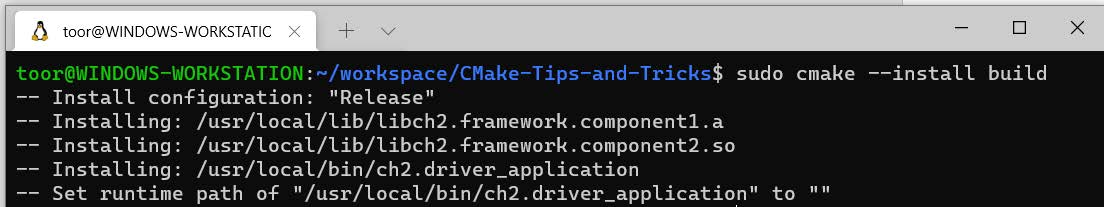
\includegraphics[width=1.\textwidth]{content/1/chapter2/images/18.jpg}\\
Figure 2.18 – Installing a project
\end{center}

The default installation directory varies between environments. For Unix-like environments, it defaults to /usr/local, whereas in a Windows environment, it defaults to C:/Program Files.

\begin{tcolorbox}[colback=webgreen!5!white,colframe=webgreen!75!black,title=Tip]
Keep in mind that the project must be already built before trying to install the project.

In order to be able to install the project successfully, you must have the appropriate rights/permissions to write to the installation target directory.
\end{tcolorbox}

\hspace*{\fill} \\ %插入空行
\noindent
\textbf{Changing the default installation path}

To change the default installation directory, you may specify the additional -{}-prefix parameter, as shown here, to change the installation directory:

\begin{tcblisting}{commandshell={}}
cmake --install build --prefix /tmp/example
\end{tcblisting}

The following figure shows the contents of the /tmp/example folder after invoking cmake -{}-install with the /tmp/example prefix:

\begin{center}
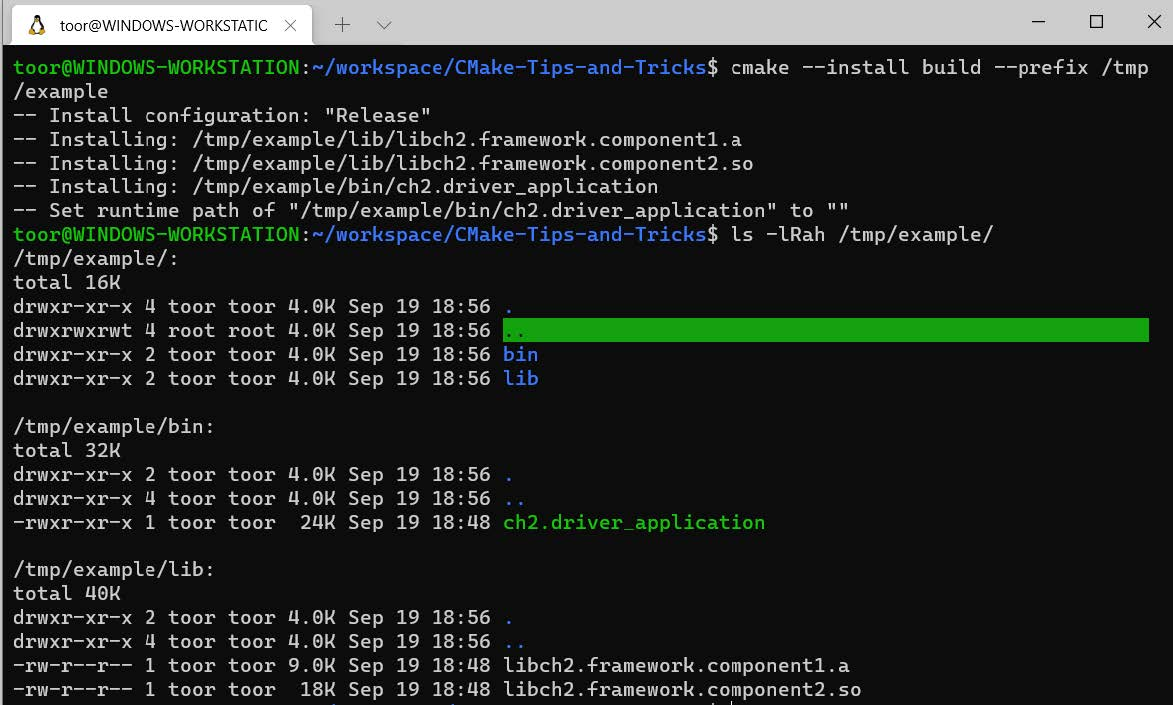
\includegraphics[width=1.\textwidth]{content/1/chapter2/images/19.jpg}\\
Figure 2.19 – Installing a project to a different path
\end{center}

As can be seen here, the installation root is successfully changed to /tmp/example.

\hspace*{\fill} \\ %插入空行
\noindent
\textbf{Stripping binaries while installing}

In the software world, build artifacts are usually bundled with some extra information, for example, a symbol table required for debugging. This information may not be necessary for executing the end product and may drastically increase binary sizes. If you're looking to reduce your end product's storage footprint, stripping binaries may be a good option. One additional benefit of stripping is that it makes it harder to reverse engineer binaries since essential symbol information is stripped away from the binaries.

CMake's -{}-install command allows the stripping of binaries while installing the operation. It can be enabled by specifying an additional -{}-strip option in the -{}-install command, as shown next:

\begin{tcblisting}{commandshell={}}
cmake --install build --strip
\end{tcblisting}

In the following example, you can observe the size difference between unstripped and stripped binaries. Note that stripping static libraries has its own limitations and CMake does not perform it by default. You can see the size of the unstripped binaries in this figure:

\begin{center}
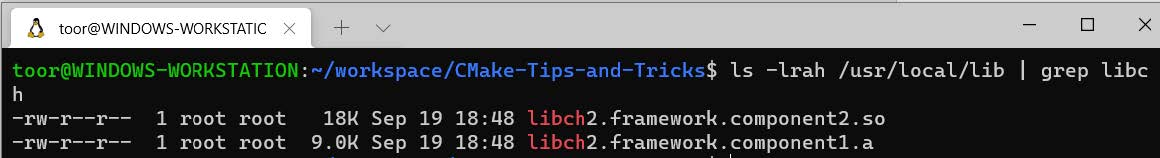
\includegraphics[width=1.\textwidth]{content/1/chapter2/images/20.jpg}\\
Figure 2.20 – Artifact size (unstripped)
\end{center}

With a stripped (cmake –install build -{}-strip) binary, the size difference looks as shown in the following figure:

\begin{center}
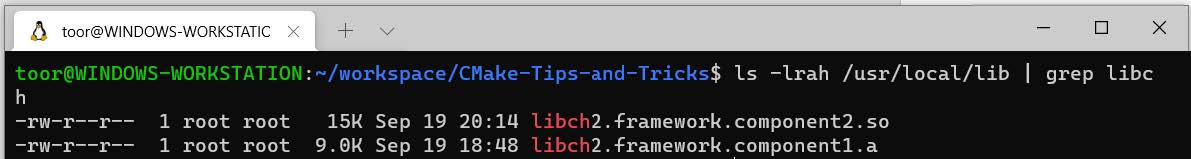
\includegraphics[width=1.\textwidth]{content/1/chapter2/images/21.jpg}\\
Figure 2.21 – Artifact size (stripped)
\end{center}

\hspace*{\fill} \\ %插入空行
\noindent
\textbf{Installing specific components only (component-based install)}

If the project is using CMake's COMPONENT feature in the install() commands, you may install specific components by specifying their component names. The COMPONENT feature allows the installation to be separated into sub-parts. For illustrating this functionality, the chapter\_2 example is structured into two components named libraries and executables.

In order to install a specific component, an additional -{}-component argument is needed along with the cmake -{}-install command:

\begin{tcblisting}{commandshell={}}
cmake --install build --component executables
\end{tcblisting}

Here is an example invocation:

\begin{center}
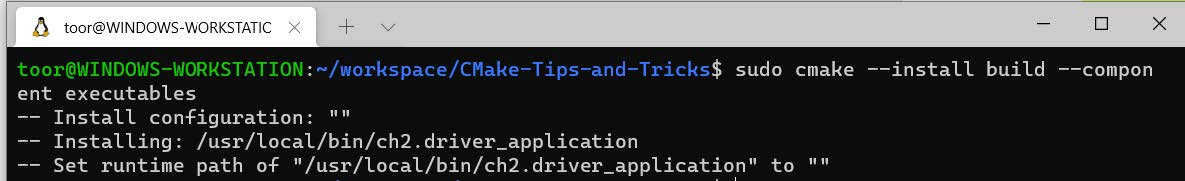
\includegraphics[width=1.\textwidth]{content/1/chapter2/images/22.jpg}\\
Figure 2.22 – Installing a specific component only
\end{center}

\hspace*{\fill} \\ %插入空行
\noindent
\textbf{Installing a specific configuration (for multiple-configuration 	generators only)}

Some of the generators support multiple configurations for the same build configuration (for example, Visual Studio). For that kind of generator, the -{}-install option provides an additional -{}-config argument to specify which configuration of binaries is intended to be installed.

Here's an example:

\begin{tcblisting}{commandshell={}}
cmake --install build --config Debug
\end{tcblisting}

\begin{tcolorbox}[colback=webgreen!5!white,colframe=webgreen!75!black,title=Note]
As you may have noticed, the command parameters used in examples are pretty long and explicit. This is intentional. Explicitly specifying arguments allows us to get consistent results in each run, no matter which environment we're running our commands in. For example, without the -G argument, CMake will default to the environment's preferred build system generator, which may not be our intention. Our motto here is, Being explicit is almost always better than being implicit. The former makes our intention clearer and naturally enables more future-proof and maintainable CMake code in CI systems/scripts as well.
\end{tcolorbox}

We have covered the fundamentals of CMake command-line usage. Let's continue to learn about the other available interface form – the graphical interface of the CMake.











